\section{Proposed Exercises.}

\subsection{Proposed exercise 1}

Let be a homogeneous and isotropic sand stratum with a thickness of
5.2 m and a permeability coefficient of $k_x=k_y=k_z=1\cdot10^{-2}$
m/s.  Underneath there is another homogeneous and isotropic stratum
formed by silty sands with a thickness of 4 meters and with a
permeability coefficient of $k_x=k_y=k_z=5\cdot10^{-5}$ m / s. Under
the silty sands there is a layer of clays that is assumed to be
impermeable. In order to reduce the filtration due to the first layer,
a sheet pile (of infinite length in the direction perpendicular to the
plane of the drawing) has been embedded, which, by execution error, has
only penetrated 4.6 m. To the left of the sheet piling (upstream) a
height of 3 meters of water has accumulated and to the right
(downstream) the runoff makes no accumulation of water. For the
problem thus defined (see Fig.~\ref{enu02}) and assuming a steady
state, answer the question you are being asked in class.
\begin{figure}[!h]
  \begin{center}
    \includegraphics[width=0.75\textwidth]{./body/images/enu02}
  \end{center}
  \caption{Model description}\label{enu02}
\end{figure}



\paragraph{NOTE:} Use the same type of elements as in the previous
solved exercise and a global mesh size of 1.4 meters.

\paragraph{HELP:} In this exercise there are two different materials
that share a common border. To reproduce it in Abaqus follow the
following steps:
\begin{itemize}
\item Create a different \textit{part} for each stratum and assign the
  corresponding material. When you are in the \textbf{Property} module
  and you are assigning a section to a \textit{part} (\textbf{Assign
    Section} command), remember not to create a \textit{set}, as shown
  in Fig.~\ref{corr01} (we want to avoid problems in the subsequent
  \textbf{Merge} operation).
  \begin{figure}[!h]
    \begin{center}
      
\includegraphics[width=0.75\textwidth]{./body/images/corr01.pdf}
    \end{center}
    \caption{\textit{Prompt} associated to \textbf{Assign Section}}
    \label{corr01}
  \end{figure}
\item In module \textbf{Assemble}, assemble a model with a dependent
  copy of each part as indicated in Fig.~\ref{ayu01}. Then press the
  command \textbf{Translate Instance} (see Fig.~\ref{ayu02}) until you
  leave them in their final position (see Fig.~\ref{ayu03}).
  \begin{figure}[!h]
    \centering
    \begin{subfigure}[!h]{0.95\textwidth}
      \includegraphics[width=\textwidth]{./body/images/ayu01}
      \caption{Initial position of the \textit{parts} copies}
      \label{ayu01}
    \end{subfigure}%
    
    % add desired spacing between images, e. g. ~, \quad, \qquad,
    % \hfill etc.
    % (or a blank line to force the subfigure onto a new line)
    \begin{subfigure}[!h]{0.15\textwidth}
      \includegraphics[width=\textwidth]{./body/images/ayu02.pdf}
      \caption{Command \textbf{Translate Instance}}
      \label{ayu02}
    \end{subfigure}%
    \begin{subfigure}[!h]{0.82\textwidth}
      \includegraphics[width=\textwidth]{./body/images/ayu03}
      \caption{Final position of the \textit{parts} copies}
      \label{ayu03}
    \end{subfigure}%
    \caption{Assemble a model with two \textit{parts} (I)}
  \end{figure}

\item Finally we try to create a new \textit{part} as the union of the
  two previous but conserving the common border between them. To do so
  press \textbf{Merge/Cut} (see Fig.~\ref{ayu02r}) making sure you
  activate the \textbf {Retain Boundary} option (see
  Fig.~\ref{ayu04}). Check that the \textit{Assembly/Instances} node
  of \textbf{Model Tree} has created the new copy (see
  Fig.~\ref{ayu05})
  \begin{figure}[!h]
    \centering
    \begin{subfigure}[!h]{0.15\textwidth}
      
\includegraphics[width=\textwidth]{./body/images/ayu02r}
      \caption{Command \textbf{Merge/Cut}}
      \label{ayu02r}
    \end{subfigure}%
    % add desired spacing between images, e. g. ~, \quad, \qquad,
    % \hfill etc.
    % (or a blank line to force the subfigure onto a new line)
    \begin{subfigure}[!h]{0.45\textwidth}
      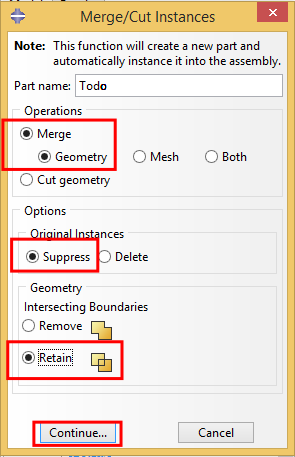
\includegraphics[width=\textwidth]{./body/images/ayu04.pdf}
      \caption{\textbf{Merge/Cut} dialog box}
      \label{ayu04}
    \end{subfigure}%
    \begin{subfigure}[!h]{0.20\textwidth}
      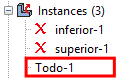
\includegraphics[width=\textwidth]{./body/images/ayu05}
      \caption{Copies from the model}
      \label{ayu05}
    \end{subfigure}%
    \caption{Assemble a model with two \textit{parts} (II)}
  \end{figure}
\item Remember that when you build the mesh you should do it on the
  new \textbf{Part} created as indicated in Fig.~\ref{ayu06}.
  \begin{figure}[!h]
    \centering
    \includegraphics[width=0.95\textwidth]{./body/images/ayu06}
    \caption{Mesh of new \textit{part}}
    \label{ayu06}
  \end{figure}

\end{itemize}
\clearpage \newpage

\subsection{Proposed exercise 2}

We have a dam with a base 27 meters wide built in concrete (which we
will assume is impermeable) of infinite length in the direction
perpendicular to the plane of the drawing. Under that base there is a
homogeneous and isotropic stratum of silty sand with a permeability
coefficient of $k_x=k_y=k_z=5\cdot10^{-5}$ m/s and a thickness of 15
m. Under this layer there is a packet of clays that we will assume are
impermeable.

A 5-meter-high membrane cut-off at the upstream edge of the dam is
built to avoid filtration and, to avoid underpressure, a 7 m long and
1 m high toe-drain with permeability of $k_x=k_y=k_z=1\cdot10^{-1}$
m/s is built too.

Upstream of the dam a height of 10 meters of water is accumulated and
downstream the runoff makes no accumulation of water. For the problem
thus defined (see Fig.~\ref{enu03}) and assuming a steady state,
answer the following questions:
\begin{enumerate}
\item Obtain the water outflow downstream (per unit length in $y$
  direction).
\item Obtain the resultant of the underpressure (vertical force) on
  the line DE per unit length in the $y$ direction.
\end{enumerate}



\begin{figure}[!h]
  \begin{center}
    \includegraphics[width=0.95\textwidth]{./body/images/enu03}
  \end{center}
  \caption{Model description}
  \label{enu03}
\end{figure}

\paragraph{NOTE:} Use the same type of elements as in the previous
solved exercise and a global mesh size of 2.5 meters. The solution to
question 1 is 1.942e-4 m$^3$/s per meter in the $y$ direction. The
solution to question 2 is 699.8 kN per meter in the $y$ direction.

\paragraph{HELP:} In this exercise there are two different materials
that share a common border. To reproduce it in Abaqus follow the steps
described in the proposed exercise 1.

\hspace{20mm}\hrulefill$\star$\hrulefill\hspace{20mm}

\clearpage \newpage
\subsection{Proposed exercise 3}

We have a dam built in concrete (which we will consider impermeable)
of infinite length in the direction perpendicular to the plane of the
drawing. Under its base there is a layer formed by two homogeneous and
isotropes materials of silty sand and under that layer there is a
packet of clays that we will assume are impermeable. A membrane
cut-off is built to reduce filtration at the upstream end of the dam
(consider the membrane 0.05 m thick). The geometry and permeability
properties of the materials are described in Fig.~\ref{enup01nn}.  We
will assume that the vertical boundaries of the stratum at the ends
are so far from the dam as to be considered impermeable. At point D we
want to simulate the effect of a pump that extracts a flow of 0.0001
m$^3$/s per linear meter in the direction $z$. To intruduce that
Neumann-type boundary condition, consult in the Abaqus' help the
command \textbf{Concentrated heat flux} (think about the sign that you
must set to simulate that we are extracting flow).  \vspace{-2mm}
\begin{figure}[!h]
  \centering
  \includegraphics[width=0.99\linewidth]{./body/images/enup01}
  \caption{Problem description}
  \label{enup01nn}
\end{figure}

Answer the questions that follow with the following considerations:
\begin{itemize}
\item Use, when defining the mesh, quadrilateral elements, mesh
  technique \textit{Free}, with a global mesh size of 1.8 meters and
  quadratic interpolation (element \textit{DC2D8}). Do not subdivide
  the parts to get a more regular mesh.
\item Consider the fluid is fresh water with density $\rho_w= 1000$
  kg/m$^3$ and the acceleration of gravity is $g=9.81$ m/s$^2$.
\item To facilitate the calculation of the underpressure, consider
  that the origin of the heights (\textit{z=0} m.) is at the base DF
  of the dam.
\end{itemize}

For the problem thus defined, calculate the outgoing flow in the
straight line GH per unit of meter in the direction $z$ (the solution
is 0.00108 m$^3$/s/ml) and the vertical force of sub-pressure under
the dam (the solution is 613.37 kN/ml). \vspace{3mm}

\hspace{20mm}\hrulefill$\star$\hrulefill\hspace{20mm}

\clearpage \newpage
\subsection{Ejercicio Propuesto 4}

Let be a soil stratum where two steel sheets (of infinite length in
the direction perpendicular to the plane of the drawing) have been
embedded. This stratum is composed of three homogeneous and isotropic
silty sand soils.  Underneath, there is a packet of clays that we will
assume is impermeable. The geometry and permeability properties of the
materials are described in Fig.~\ref{enup04}.  To the left of sheet
pile 1, a volume of water with a constant height above the H point of
15 meters is accumulated.  Between sheet piles 1 and 2 we build a
concrete plate that makes the CD contour impermeable.  To the right of
sheet pile 2 there is a network of injectors that apply a flow of
value $q=10^{-3}$ m$^3$/m$^2$/s in the EF contour (positive indicates
flow into the surface).  Finally, in the FG contour, runoff provoques
that water does not accumulate above the ground. We will assume that
the vertical borders of the stratum at the ends are so far away from
the sheet piles as to be considered impermeable.

\vspace{-2mm}
\begin{figure}[!h]
  \centering
  \includegraphics[width=1.0\linewidth]{./body/images/enup04}
  \caption{Problem description}
  \label{enup04}
\end{figure}

Use the following considerations (since it is a plane problem, we will
take a unit thickness and the values of flow and force will be per
meter in the $ z $ direction):
\begin{itemize}
\item When defining the mesh quadrilateral elements, use meshing
  technique \textit{Free}, with global mesh size 1.3 meters and linear
  interpolation (the element type should be \textit{DC2D4}). Do not
  subdivide the parts to obtain a more regular mesh.
\item Consider the fluid is fresh water with density $\rho_w=1000$
  kg/m$^3$ and that the acceleration of gravity is $ g = 9.81 $
  m/s$^2$.
\item The line that separates materials 1 and 3 is vertical.
\item \textbf{Use as the origin of geometric heights the horizontal
    line that passes through H.}
\end{itemize}

For the problem described and assuming a steady state, calculate the
vertical force of underpressure under the CD block (1454.8 kN), the pore pressure
of the fluid at point A (170.6 kPa), the total head of point B (2.67 m), the
modulus of the flow vector at the centroid of the element E1 ($9.62\cdot 10^{-5}$ m$^3$/m$^2$/s) and the
flow through the straight line BI (0.00275 m$^3$/s).
